% main.tex
%--------------------------------------------------------------------------------------------------------------
% Vorlage Bachelor-/ Master-Thesis laut Vorgaben der Hochschule Wismar, Fakultät für Ingenieurwissenschaften
% Überarbeitete Version von Prof. Dr. Manfred Krüger vom 17.03.2010
%--------------------------------------------------------------------------------------------------------------
% Author:               Florian Drews
% Erstellt am:          11. Februar 2015
% Zuletzt geändert am:  11. Februar 2015
%--------------------------------------------------------------------------------------------------------------

%--------------------------------------------------------------------------------------------------------------
% header.tex
%--------------------------------------------------------------------------------------------------------------

%--------------------------------------------------------------------------------------------------------------
% Art des Dokumentes, Layout, Papierformat, Schriftgröße
%--------------------------------------------------------------------------------------------------------------
\documentclass[12pt,					              % Grundschriftgöße
							 oneside,				              % einseitiges Dokument
							 a4paper,				              % Papiergröße
							 toc=listof,		              % Verzeichnis (Abbildungen etc.) in das Inhaltsverzeichnis
							 toc=bibliography,			      % Literaturverzeichnis ins Inhaltsverzeichnis
							 fleqn,					              % Mathematische Formeln linksbündig darstellen
							 numbers=noenddot,
							 headsepline]	          % Punkt am Ende der Nummerierung des Inhaltsverzeichnisses entfernen
							 {scrreprt}

%--------------------------------------------------------------------------------------------------------------
% Daten für die Titelseite
%--------------------------------------------------------------------------------------------------------------
\title{\Kategorie}
\author{\Verfasser}
\date{\today{}}
							 
%--------------------------------------------------------------------------------------------------------------
% Schriftarten anpassen
%--------------------------------------------------------------------------------------------------------------
\setkomafont{sectioning}{\rmfamily\bfseries}					% Titelzeilen
\setkomafont{caption}{\small}													% Schrift für Caption
\setkomafont{captionlabel}{\sffamily\bfseries\small}	% Schrift für 'Abbildung'
\setkomafont{chapterentry}{\small\bfseries}						% Schrift für Inhaltsverzeichnis
\setkomafont{chapter}{\large\bfseries}								% Schrift für Kapitel
\setkomafont{section}{\normalsize}										% Schrift für Section
\setkomafont{subsection}{\normalsize}									% Schrift für Subsection
							 
%--------------------------------------------------------------------------------------------------------------
% Konstanten festlegen 
%--------------------------------------------------------------------------------------------------------------
\newcommand{\Kategorie}{Bachelor-Thesis}
\newcommand{\Titel}{Untersuchung des ETL-Tools Tensei-Data und dessen Einsatz im Prozess der Datenmigration bei der SIV.\@AG}
\newcommand{\Verfasser}{Martin Pohl}
\newcommand{\Geburtstag}{13. April 1981}
\newcommand{\Geburtsort}{Rostock}
\newcommand{\Betreuer}{Prof. Dr.-Ing. Antje Raab-D\"usterh\"oft}
\newcommand{\ZweitBetreuer}{Betriebswirt (VWA) Detlef Herold}

%--------------------------------------------------------------------------------------------------------------
% benötigte Pakete
%--------------------------------------------------------------------------------------------------------------
\usepackage[utf8]{inputenc}             % Zeichensatzkodierung. Direkte Angabe von Umlauten im Dokument. 
\usepackage[english, ngerman]{babel}    % Deutsche und Englische Sprachanpassung
\usepackage[T1]{fontenc}                % Silbentrennung bei Sonderzeichen
\usepackage{lmodern}					          % bietet neuere Schriften, sieht besser aus im Acrobat Reader
\usepackage{graphicx}                   % einfaches Einbinden von Grafiken
\usepackage{subfigure}				          % erweiterte Darstellung von Bildern
\usepackage{listings}                   % ermöglicht Einbinden von Quelltexten
\usepackage{amsmath,amssymb}	          % erweiterter Formelsatz und zusätzliche Mathe-Symbole
\usepackage{booktabs}					          % professionelle Tabellen setzen, typographisch richtig
\usepackage{shortvrb}					          % benutzen der Verbatim-Umgebung, stellt Quelltexte exakt da
\usepackage{setspace}					          % Package zum Kontrollieren von Leerräumen
\usepackage{color,moreverb}		          % Farben
\usepackage{scrhack}                    % behebt Warnungen die mit float und dem Koma-Skript zu tun haben
\usepackage{blindtext}                  % zum Einbinden von Blindtexten
\usepackage[plainheadsepline, nouppercase,]{scrpage2}                   % Koma-Skript konforme Möglichkeit Kopf- und Fußzeile anzupassen
\usepackage{graphicx}
\usepackage{url}
\usepackage{tabularx}


%--------------------------------------------------------------------------------------------------------------
% Definition Seitenränder
%--------------------------------------------------------------------------------------------------------------
\usepackage[left=3cm,					  % linker Rand
						right=3cm,				  % rechter Rand
						top=1.5cm,				  % oberer Rand
						bottom=1.5cm,			  % unterer Rand
						includeheadfoot,	  % bezieht die Kopf- und Fußzeile mit ein
						bindingoffset=0cm,]	% Bundsteg
						{geometry}

%--------------------------------------------------------------------------------------------------------------
% Metadaten für die PDF-Erzeugung
%--------------------------------------------------------------------------------------------------------------
\usepackage[pdftex,
						pdfauthor={\Verfasser},	                                    % Name des Autors
						pdftitle={\Titel},			                                    % Name der Arbeit
						pdfcreator={Latexmk, KOMA-Script},                          % Von was erzeugt
						pdfsubject={\Kategorie},	                                  % Was für eine Arbeit ist es
						pdfkeywords={\Titel},
						plainpages=false,
						hypertexnames=false,
						pdfpagelabels]{hyperref}

%--------------------------------------------------------------------------------------------------------------
% Farbe für Links in PDF-Dokumenten definieren
%--------------------------------------------------------------------------------------------------------------
\definecolor{LinkColor}{rgb}{0,0,0.5}	% Festlegen einer neuen Farbe

\hypersetup{colorlinks=true,			% farbliche Links
						breaklinks=true,			% Zeilenumbruch erlauben
						linkcolor=black,			% Farbe für interne Links
						citecolor=black,			% Farbe für Links zum Literaturverzeichnis
						filecolor=LinkColor,	% Farbe für externe Dateilinks
						menucolor=LinkColor,	%
						urlcolor=LinkColor}		% Farbe für externe Links

%--------------------------------------------------------------------------------------------------------------
% Darstellung des Literaturverzeichnisses einstellen
%--------------------------------------------------------------------------------------------------------------
\bibliographystyle{alphadin}	% Stil des Literaturverzeichnisses (hier nach DIN 1505)

%--------------------------------------------------------------------------------------------------------------
% Darstellung des Glossars und des Abkürzungsverzeichnisses einstellen
%--------------------------------------------------------------------------------------------------------------
\usepackage[nomain,style=listdotted,nonumberlist,acronym,toc]{glossaries}
\usepackage{glossary-longragged}
\renewcommand{\glspostdescription}{}        % Punkt am Ende der vollständigen Beschreibung entfernen
%\loadglsentries{verzeichnisse/abkuerzungen} % Alternativdatei für die Definition der Abkürzungen
\makeglossaries
\newacronym{erp}{ERP}{Enterprise Resource Planning}

\newacronym{etl}{ETL}{Extraction, Transformation, Loading}

\newacronym{dbms}{DBMS}{Datenbank-Management-System}

\newacronym{plsql}{PL/SQL}{Procedural Language/Structured Query Language}

\newacronym{rdbms}{RDBMS}{Relational Database Management System}




\newacronym{lan}{LAN}{Local Area Network}

\newacronym{din}{DIN}{Deutsches Institut für Normung}

\newacronym{iso}{ISO}{International Standards Organization}

\newacronym{ieee}{IEEE}{Institute of Electronic and Electrotechnical Engineers}

\newacronym{svm}{svm}{support vector machine}

\newacronym{vcs}{VCS}{Version Control System}

\newacronym{swe}{SWE}{Softwareentwicklung}

\newacronym{ide}{IDE}{integrierte Entwicklungsumgebung}

\newacronym{gui}{GUI}{Graphical User Interface}

\newacronym{url}{URL}{Uniform Resource Locator}

\newacronym{www}{WWW}{World Wide Web}

\newacronym{http}{HTTP}{Hyper Text Transfer Protocol}

\newacronym{cwi}{CWI}{Centrum voor Wiskunde en Informatica}

\newacronym{gpl}{GPL}{General Public License}

\newacronym{ocr}{OCR}{optische Zeichenerkennung}

\newacronym{xml}{XML}{Extensible Markup Language}

\newacronym{html}{HTML}{Hypertext Markup Language}

\newacronym{xmlp}{XMLP}{XML Path Language}

\newacronym{dom}{DOM}{Document Object Model}

\newacronym{sax}{SAX}{Simple API for XML}

\newacronym{uic}{UIC}{Qt user interface compiler}
				% die Datei abkürzungen.tex zum Verwalten der Abkürzungen verwenden
%--------------------------------------------------------------------------------------------------------------
% Abbildung in Bild umbenennen
%--------------------------------------------------------------------------------------------------------------
\addto{\captionsngerman}{
	\renewcommand*{\figurename}{Bild}}
	
	
\DeclareGraphicsExtensions{.pdf,.png,.jpg}

%--------------------------------------------------------------------------------------------------------------
% Quellcodeformatierung
%--------------------------------------------------------------------------------------------------------------

\lstloadlanguages{Matlab,[Visual]C++,C, Python}

%\definecolor{lbcolor}{white}{0.9}			% Farbe für den Hintergrund definieren				
\definecolor{darkblue}{rgb}{0,0,.6}		% Farbe für Schlüsselwörter
\definecolor{darkred}{rgb}{.6,0,0}		% Farbe für Strings
\definecolor{darkgreen}{rgb}{0,.6,0}	% Farbe für Kommentare

%\lstset{language=Matlab,					% Programmiersprache der Listings
%				numbers=left,							% Zeilennummern links angeben
%				stepnumber=1,							% in welchem Abstand sollen Zeilennummern angeben werden (1 2 3..)
%				numbersep=5pt,
%				numberstyle=\tiny,				% grösse der Nummern
%				breaklines=true,					% Zeilenumbruch zulassen
%				breakautoindent=true,
%				postbreak=\space,
%				tabsize=2,								% Tabulator auf 2 setzen
%				basicstyle=\ttfamily\footnotesize,
%				showspaces=false,					% leerzeichen nicht anzeigen
%				showstringspaces=false,		% keine Leerzeichen bei Strings anzeigen
%				extendedchars=true,
%				backgroundcolor=\color{lbcolor}}	% Hintergrundfarbe des Listings

\lstset{language=Python,								% Programmiersprache der Listings
				%alsolanguage=Matlab,			% alternative Programmiersprache der Listings
				frame=none,								% keinen Rahmen
				frameround=ffff,					% wenn ein Rahmen dargestellt werden soll, sind die Ecken spitz
				captionpos=b,							% Position der Benennung
				numbers=left,							% Zeilennummern links angeben
				stepnumber=1,							% in welchem Abstand sollen Zeilennummern angeben werden (1 2 3..)
				numbersep=5pt,						% Abstand zwischen Nummerierung und Listing
				numberstyle=\tiny,				% grösse der Nummern
				breaklines=true,					% Zeilenumbruch zulassen
				breakautoindent=true,
				postbreak=\space,
				tabsize=4,								% Tabulator auf 4 setzen
				escapechar=\$,
				basicstyle=\scriptsize\ttfamily,
				keywordstyle=\color{darkblue}\bfseries\ttfamily,	% Darstelung der Schlüsselwörter
				stringstyle=\ttfamily\color{darkred},  						% Darstellung der Strings
				commentstyle=\itshape\color{darkgreen},						% Darstellung der Kommentare
				showspaces=false,					% leerzeichen nicht anzeigen
				showstringspaces=false,		% keine Leerzeichen bei Strings anzeigen
				xleftmargin=.52cm,
				xrightmargin=.52cm,				
				backgroundcolor=\color{white}}	% Hintergrundfarbe des Listings}

%--------------------------------------------------------------------------------------------------------------
% Darstellung Kopf- und Fußzeile einstellen
%--------------------------------------------------------------------------------------------------------------

\pagestyle{scrheadings}
\automark[chapter]{chapter}
\clearscrheadfoot
\renewcommand{\headfont}{\normalfont}
\renewcommand*{\chaptermarkformat}{\chapapp\ \thechapter.\ \ }% Nummer in Kopfzeile verschwindet
\rohead[\headmark]{\headmark}
\rofoot[\pagemark]{\pagemark}
    % Header-Datei einfügen --> beinhaltet sämtliche Vorgaben

%--------------------------------------------------------------------------------------------------------------
% Beginn des Dokumentes --> Hauptdatei zum kompilieren
%--------------------------------------------------------------------------------------------------------------

\begin{document}                   

  %-----------------------------------------------------------------------------
	% Titelseite
	%-----------------------------------------------------------------------------
  %--------------------------------------------------------------------------------------------------------------
% titel.tex - Titelseite
%--------------------------------------------------------------------------------------------------------------

\begin{titlepage}
	\setlength\headsep{-5mm}
	\begin{figure}[!h]
		\begin{minipage}{0.8\textwidth}
			\textbf{Hochschule Wismar} \\
			University of Applied Sciences \\
			Technology, Business and Design \\
			Fakultät für Ingenieurwissenschaften, Bereich EuI \\
		\rule{\textwidth}{0.5pt}
		\end{minipage}
		\begin{minipage}[r]{0.1\textwidth}
			\begin{flushright}
				
\includegraphics[height=6\baselineskip]{bilder/hs-wismar_logo-fiw.jpg}\hfuzz=25pt %hfuzz verhindert Warnung "Overfull \hbox "
			\end{flushright}
		\end{minipage}
	\end{figure}
	\vspace*{6cm}
	\begin{center}
		\Huge
		\textbf{\Kategorie}  \\
		\vspace{2cm}
		\large \Titel
		\begin{table*}[b]
			\begin{tabular}{rl}
				Eingereicht am: & \today \\
				\\
				von: & \Verfasser \\
				& geboren am \Geburtstag \\
				& in \Geburtsort
			\end{tabular}
		\end{table*}
	\end{center}
\end{titlepage}
               % Einbinden der Titelseite 
  \onehalfspacing 					            % 1 1/2-zeilig (package 'setspace'
  %-----------------------------------------------------------------------------
	% Aufgabenstellung, Zusammenfassung/Abstract
	%-----------------------------------------------------------------------------
	%--------------------------------------------------------------------------------------------------------------
% kapitel/aufgabenstellung.tex
%--------------------------------------------------------------------------------------------------------------


\section*{Aufgabenstellung}
Einfügen der ausgegebenen Aufgabenstellung der Bachelor-Thesis. Der Titel der Arbeit wird bei deutschsprachigen Titeln in der englischen Fassung wiederholt.
\newpage
	% Aufgabenstellung einfügen
	%--------------------------------------------------------------------------------------------------------------
% kapitel/zusammenfassung.tex
%--------------------------------------------------------------------------------------------------------------

\section*{Zusammenfassung}
Hier sollte auf max. $1/2$ bis $3/4$ Seiten eine Zusammenfassung erstellt werden. 
\begin{itemize}
	\item Motivation, Einordnung, Umfeld und Abgrenzung der Arbeit
	\item wesentliche Schwerpunkte und Ergebnisse der Arbeit
\end{itemize}
\vspace{0.5cm}

\section*{Abstract}
English Version.
		% Zusammenfassung und englischen Abstract einfügen
	
	%-----------------------------------------------------------------------------
	% Inhaltsverzeichnis
	%-----------------------------------------------------------------------------
  %--------------------------------------------------------------------------------------------------------------
% verzeichnisse/inhaltsverzeichnis.tex
%--------------------------------------------------------------------------------------------------------------

\pdfbookmark[1]{Inhaltsverzeichnis}{toc}	% Inhaltsverzeichnis zu den Lesezeichen hinzufügen
\singlespacing 						% 1-zeilig
\tableofcontents 					% Inhaltverzeichnis einfügen
\onehalfspacing 					% 1 1/2-zeilig (package 'setspace')

	
	%-----------------------------------------------------------------------------
	% Hauptteil
	%-----------------------------------------------------------------------------
	%--------------------------------------------------------------------------------------------------------------
% kapitel/einleitung.tex
%--------------------------------------------------------------------------------------------------------------

\chapter{Einleitung}
max. 2--3 Seiten
\begin{itemize}
	\item Einführung in die Thematik und das wissenschaftlich-technische Umfeld
 	\item Einordnung in das Wissenschaftsgebiet / tangierte Gebiete
 	\item Analyse der Aufgabenstellung (Problemerfassung)
 	\item Realisierungsumfeld und Randbedingungen
\end{itemize}
				% Einleitung einbinden
	%--------------------------------------------------------------------------------------------------------------
% kapitel/grundlagen.tex
%--------------------------------------------------------------------------------------------------------------

\chapter{Theoretische Grundlagen}

In diesem Kapitel werden zunächst die Grundlagen und Begrifflichkeiten vorgestellt. Weiterhin werden die Kriterien für eine erfolgreiche Migrationen erläutert.

\section{SIV.AG}\label{SIV.AG}

Die SIV.AG ist ein Anbieter für ganzheitliche Lösungen im Bereich der deutschen und internationalen Energie- und Wasserwirtschaft. Das Kernstück vom Unternehmen ist das Softwareprodukt kVASy$^\text{\textregistered}$, ein vollständig integriertes \acrfull{erp}, welches insbesondere auf die Anforderungen und Prozesse der Energie- und Wasserwirtschaft ausgerichtet ist. Das Unternehmen wurde 1990 durch Jörg Sinnig als Software- und Beratungshaus gegründet. Zum gegenwärtigen Zeitpunkt beschäftigt die SIV.AG mehr als 400 Mitarbeiter. Ihr Leistungsportfolio reicht von der Beratung und Analyse über die Implementierung und Bereitstellung der IT-Systeme bis hin zur Datenmigration, Schulung und Pflege.\cite{SIV13}

\section{kVASy\texorpdfstring$^\text{\textregistered}$}

Das zuvor bereits erwähnte kVASy$^\text{\textregistered}$ ist ein webbasiertes \acrshort{erp} und bildet das Aushängeschild der SIV.AG. Zu der Produktfamilie gehören die 4 Bereiche Finance (Buchaltung), Billing (Abrechnung) und EDM (Vertragsverwaltung), Technical Assets (Anlagenmanagement) und xRM (Kundenbeziehungsmanagement).

\section{Datenbanksysteme}
\subsection{Elemente eines relationalen Datenbanksystems}
\subsection{Beziehungen und Normalformen}
\subsection{Schema}

\section{Datenintegration/Datenmigration}

\section{Transformationen}

\section{ETL-Tools}

\section{Qualitätskontrolle/Protokollierung}

\section{Kriterien für erfolgreiche Migrationen}
\begin{itemize}

  \item Ziele einer Migration
  \item Vorgehensweise/Migrationsplanung
  \item Strategische Aspekte
  \item Rechtliche Aspekte
  \item Wirtschaftliche Aspekte
  \item Qualitative Aspekte
  \item Aspekte des Systembetriebs
  \item Organisatorische Aspekte
  \item Sicherheitsaspekte
\end{itemize}
\subsection{Ziele einer Migration}
Bevor es zur einer 
\begin{itemize}
  \item ein verbesserter Anwendernutzen
  \item das Herstellen eines rechtlich notwendigen Zustands
  \item die Behebung von Fehlern
  \item die Erweiterung des Funktionsumfangs
  \item eine verbesserte Integration in die vorhandenen Softwaresysteme
  \item eine verbesserte Interoperabilität
  \item eine Verringerung der laufenden Kosten
  \item die Erhöhung der Produktivität
  \item die bessere Nutzung vorhandener Resourcen
  \item die Einhaltung strategischer Vorgaben
\end{itemize}
\subsection{Wirtschaftliche Aspekte}
\subsection{Qualitative Aspekte}
\subsection{Organisatorische Aspekte}
\subsection{Vorgehensweise/Migrationsplanung}
\subsection{Anforderung an die Datenmigration}


% \subsection{Bilder}
% Beispiel für ein Bild in \LaTeX{}
% \begin{figure}[ht]
% 	\begin{center}
% 		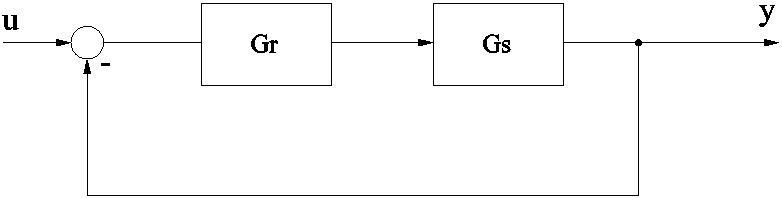
\includegraphics[scale=0.3]{bilder/regelkreis.png}
% 		\caption{Ein Standard-Regelkreis}
% 		\label{pic:grund:regelkreis}
% 	\end{center}
% \end{figure}

% \subsection{Tabellen}
% Beispiel für eine Tabelle in \LaTeX{}
% \begin{table}[ht]
% 	\begin{center}
% 		\caption{Verwendete Matrizen}
% 		\begin{tabular}{|l|l|l|}
% 			\hline
% 			Matrix& Dimension& Symbol\\
% 			\hline
% 			Systemmatrix& $n\times n$& \textrm{A}\\
% 			\hline
% 			Ausgangsmatrix& $m\times n$& \textrm{C}\\
% 			\hline
% 		\end{tabular}
% 		\label{tab:grund:matrizen}
% 	\end{center}
% \end{table}
% 
% \subsection{Formeln}
% Beispiel für eine Formel in \LaTeX{}
% \begin{equation}
% 	c^2 = a^2 + b^2
% \end{equation}
% und noch eine Formel
% \begin{equation}
% 	f_1(x) = x_1 + x_2 + x_3
% \end{equation}
% Für weitere Möglichkeiten Formeln in \LaTeX{} einzufügen, schauen sie bitte in \cite{Peters2005}.
% 
% \subsection{{Bib\TeX}}
% Bib\TeX{} ermöglicht das erstellen eines Literaturverzeichnisses. Für die die sich weiter einarbeiten wollen, empfehle ich folgende Seite \cite{wiki:bibtex}.
% 
% \subsection{Abkürzungen}
% Es wird das Package \textit{glossary} verwendet. Mit ihm ist es möglich ein Abkürzungsverzeichnis und ein Glossary zu erstellen. Beispiel: \acrfull{lan} \acrfull{www}
				% Grundlagen Kapitel einfügen (grund.tex)
	%--------------------------------------------------------------------------------------------------------------
% kapitel/schluss.tex
%--------------------------------------------------------------------------------------------------------------

\chapter{Bewertung, Zusammenfassung und Ausblick}


\section{Bewertung}
\section{Ausblick}
\section{Zusammenfassung}

%Neben einer kurzen Zusammenfassung der wichtigsten Ergebnisse, soll in diesem Abschnitt auf weitere Fragestellungen oder noch offene, durch die Arbeit aufgeworfene Probleme, hingewiesen werden (Umfang max. 2-3 Seiten).
						% Schlusskapitel einfügen (schluss.tex)
	
	%-----------------------------------------------------------------------------
	% Literaturverzeichnis einfügen, 
	% Nutzung der BibTeX-Technologie --> literatur.bib 
	%-----------------------------------------------------------------------------
	%\nocite{*}								              % Für diejenigen die alle Einträge die in Literatur.bib stehen auch verarbeitet haben möchten, ansonsten werden nur die Einträge/Verweise verwendet die auch im Text verwendet werden  
	\bibliography{verzeichnisse/literatur}	% gibt Datei mit der Literatur an
	
	%-----------------------------------------------------------------------------
	% Verzeichnisse
	%-----------------------------------------------------------------------------
	\singlespacing 						          % 1-zeilig
	\listoffigures						          % Bildverzeichnis einfügen
	\listoftables							          % Tabellenverzeichnis einfügen
	\printglossary[type=\acronymtype, title=Abkürzungsverzeichnis, toctitle= Abkürzungsverzeichnis, style=super]
	
	%-----------------------------------------------------------------------------
	% Anhänge z.B. Quellcodebeispiele
	%-----------------------------------------------------------------------------
	
	%%--------------------------------------------------------------------------------------
% kapitel/anhang.tex
%--------------------------------------------------------------------------------------

%--------------------------------------------------------------------------------------
% Anhang
%--------------------------------------------------------------------------------------
\appendix
% Auch hier sind Gliederungen aller \chapter, \section
\chapter{Auflistung von Quellcode und ähnliches}

	
	%-----------------------------------------------------------------------------
	% Selbstständigkeitserklärung und Thesen
	%-----------------------------------------------------------------------------
	
	%--------------------------------------------------------------------------------------
% kapitel/selbstständigkeitserklärung.tex
%--------------------------------------------------------------------------------------

%--------------------------------------------------------------------------------------
% Selbstständigkeitserklärung sehr wichtig
%--------------------------------------------------------------------------------------
\chapter*{Selbstständigkeitserklärung}
\addcontentsline{toc}{chapter}{Selbstständigkeitserklärung}
\rohead[Selbstständigkeitserklärung]{Selbstständigkeitserklärung} % rechts oben in der Kopfzeile Chapter darstellen
Hiermit erkläre ich, dass ich die hier vorliegende Arbeit selbstständig,
ohne unerlaubte fremde Hilfe und nur unter Verwendung der aufgeführten
Hilfsmittel angefertigt habe.

\begin{tabular}{p{6cm}p{7cm}}
	\\
  \\
  \\
  \\
  Ort, Datum& Unterschrift
\end{tabular}

	
	%--------------------------------------------------------------------------------------
% kapitel/thesen
%--------------------------------------------------------------------------------------

\newpage
\hypertarget{Thesen}{}
\pdfbookmark[0]{Thesen}{Thesen}	% Thesen zu den Lesezeichen hinzufügen
\thispagestyle{empty}						% keine Kopf- oder Fusszeile
\begin{large}
	\textbf{Thesen} \\ \\
\end{large}
\textbf{Bachelor-Thesis} \\
\textbf{\Titel} \\
\begin{table}[htp]
		\begin{tabular}{rl}
			Eingereicht am: & \today \\
				\\
				von: & \Verfasser \\
				& geboren am \Geburtstag \\
				& in \Geburtsort \\
				\\
				Betreuer: & \Betreuer \\
				2. Prüfer: & \ZweitBetreuer
		\end{tabular}
\end{table}
\begin{enumerate}
	\item kurze Stichpunktartige Auflistung Diskussionswürdiger Punkte der Diplomarbeit
	\item hier eine weitere These
\end{enumerate}


\end{document}
